% VDE Template for EUSAR Papers
% Provided by Barbara Lang und Siegmar Lampe
% University of Bremen, January 2002
% English version by Jens Fischer
% German Aerospace Center (DLR), December 2005
% Additional modifications by Matthias Wei{\ss}
% FGAN, January 2009

%-----------------------------------------------------------------------------
% Type of publication
\documentclass[a4paper,10pt]{article}
%-----------------------------------------------------------------------------
% Other packets: Most packets may be downloaded from www.dante.de and
% "tcilatex.tex" can be found at (December 2005):
% http://www.mackichan.com/techtalk/v30/UsingFloat.htm
% Not all packets are necessarily needed:
\usepackage[T1]{fontenc}
\usepackage[latin1]{inputenc}
%\usepackage{ngerman} % in german language if required
\usepackage[nooneline,bf]{caption} % Figure descriptions from left margin
\usepackage{times}
\usepackage{multicol}
\usepackage{amsmath}
\usepackage{amssymb}
\usepackage[dvips]{graphicx}
\usepackage{epsfig}
\input{tcilatex}
%-----------------------------------------------------------------------------
% Page Setup
\textheight24cm \textwidth17cm \columnsep6mm
\oddsidemargin-5mm                 % depending on print drivers!
\evensidemargin-5mm                % required margin size: 2cm
\headheight0cm \headsep0cm \topmargin0cm \parindent0cm
\pagestyle{empty}                  % delete footer and header
%----------------------------------------------------------------------------
% Environment definitions
\newenvironment*{mytitle}{\begin{LARGE}\bf}{\end{LARGE}\\}%
\newenvironment*{mysubtitle}{\bf}{\\[1.5ex]}%
\newenvironment*{myabstract}{\begin{Large}\bf}{\end{Large}\\[2.5ex]}%
%-----------------------------------------------------------------------------
% Using Pictures and tables:
% - Instead "table" write "tablehere" without parameters
% - Instead "figure" write "figurehere " without parameters
% - Please insert a blank line before and after \begin{figuerhere} ... \end{figurehere}
%
% CAUTION:   The first reference to a figure/table in the text should be formatted fat.
%
\makeatletter
\newenvironment{tablehere}{\def\@captype{table}}{}
\newenvironment{figurehere}{\def\@captype{figure}\vspace{2ex}}{\vspace{2ex}}
\makeatother



%%%%%%%%%%%%%%%%%%%%%%%%%%%%%%%%%%%%%%%%%%%%%%%%%%%%%%%%%%%%%%%%%%%%%%%%%%%%%%
\begin{document}

% Please use capital letters in the beginning of important words as for example
\begin{mytitle}Pedometer for STM32F4\end{mytitle}
\begin{mysubtitle}Use the MEMS accelerometer to count number of steps\end{mysubtitle}
%
% Please do not insert a line here
%
\\
De Donatis Emanuele\\
Matr. 817667, (emanuele.dedonatis@mail.polimi.it)\\
\hspace{10ex}
Pistone Bruno\\
Matr. 818949, (bruno.pistone@mail.polimi.it)\\
\begin{flushright}
\emph{Report for the master course of Embedded Systems}\\
\emph{Reviser: PhD. Patrick Bellasi (bellasi@elet.polimi.it)}
\end{flushright}

Received: November, 04 2013\\
\hspace{10ex}

\begin{myabstract} Abstract \end{myabstract}
This project is part of a collaborative project whose purpose is to develop a simple 
yet realistic training support system. The goal of this project is to develop a pedometer 
using the MEMS motion sensor on the STM32F4DISCOVERY board. The device provides
the user with statistics about its training activity.

\vspace{4ex}	% Please do not remove or reduce this space here.
\begin{multicols}{2}

%%%%%%%%%%%%%%%%%%%%%%%%%%%%%%%%%%%%%%%%%%%%%%%%%%%%%%%%%%%%%%%%%%%%%%%%%%%%%
\section{Introduction}
During the Real-Time Operating System course of the Polytechnic of Milan has been
proposed a collaborative project whose aim is to develop a Personal Trainer device
based on the economical development board STM32F4DISCOVERY and the 
RTOS Miosix embedded OS. 

Each group was assigned one of the following modules
\begin{center}
\begin{tabular}{|l|c|r|} \hline
{\bf Module Name} & {\bf Device}\\ \hline
Pedometer & MEMS \\
User Interface & UART, Flash\\
Audio Feedback & CS43L22 (DAC) \\
Voice Commands & NONE (PCM Samples) \\
PCM Encoding & MP45DT02 MEMS Mic\\
Social Wireless & NRF24L01 2.4GHz TxRx\\
Context Awareness & ADC \\ \hline
\end{tabular}
\end{center}

The final goal is to join each module in order to build a working system.

%-----------------------------------------------------------------------------
\subsection{MEMS Motion Sensor}
% Please avoid separations in titles
% and separate text manually

The STM32F4DISCOVERY includes the LIS302DL ST MEMS motion sensor.
It is an ultra compact low-power three-axis linear accelerometer. It includes
a sensing element and an IC interface able to provide the measured acceleration
to the external world through I2C/SPI serial interface.\cite{Norman09Learn}

The STM32F4 controls this motion sensor through the SPI interface (see {\bf Figure
\ref{fig:LIS302DL}}). 

\begin{figurehere}
 \centering
 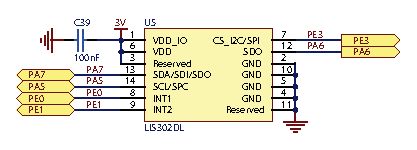
\includegraphics[width=8cm, height=3cm]{./eps/LIS302DL.eps}
 \caption{LIS302DL Motion Sensor}
 \label{fig:LIS302DL}
\end{figurehere}


%-----------------------------------------------------------------------------
\subsection{The second subsection of the first \\ Section}

Lorem ipsum dolor sit amet, consectetur adipiscing elit. Donec et ligula. Nullam
in libero. Donec dictum pede in justo. Lorem ipsum dolor sit amet, consectetur
adipiscing elit. Aliquam congue. Aliquam egestas. Nunc eu est ac nibh mattis
vestibulum. Curabitur aliquet bibendum odio. Etiam hendrerit. Nunc a velit quis
dui molestie consequat. Sed et turpis et mi feugiat tincidunt. Sed sollicitudin.
Ut risus? Duis eget orci eu turpis consectetur fringilla? Lorem ipsum dolor sit
amet, consectetur adipiscing elit. Nullam tellus ligula, placerat vitae, tempor
vitae, varius id; est! Nullam et ipsum eget tellus eleifend sollicitudin? Fusce
urna massa, imperdiet vitae, convallis in; lacinia sed, tortor.

\begin{figure*}[t]
  \centering
 \includegraphics[width=16cm, height=4cm]{./eps/placeholder.eps}
 \caption{Some wide-figure caption.}
 \label{fig:myfigure2}
\end{figure*}

And this is the reference to a single column figure (see {\bf Figure
\ref{fig:myfigure2}}). Lorem ipsum dolor sit amet, consectetur adipiscing elit.
Nullam consectetur neque at orci. Curabitur non metus. Praesent congue porta
nisl. Suspendisse ultricies, sem ac ultrices aliquam, erat nisi fermentum est; a
rhoncus mauris arcu eget nibh. Aliquam sollicitudin velit non erat. Lorem ipsum
dolor sit amet, consectetur adipiscing elit. Integer nulla diam, facilisis vel,
accumsan sed; molestie egestas, massa. Fusce malesuada, ipsum et pulvinar
aliquet, est dolor laoreet enim, quis porttitor erat mauris eget sapien. Integer
vitae urna. Duis lectus.

%%%%%%%%%%%%%%%%%%%%%%%%%%%%%%%%%%%%%%%%%%%%%%%%%%%%%%%%%%%%%%%%%%%%%%%%%%%%%
\section{The Second Section}

Lorem ipsum dolor sit amet, consectetur adipiscing elit.  Aenean magna. Nunc non
ante eget nibh condimentum tempor. Nullam ullamcorper lectus eget mauris. Nam
neque orci; rhoncus at, pulvinar quis, elementum sit amet, turpis. Mauris
posuere nisi ut justo. Morbi non lorem vitae mauris interdum faucibus.
Vestibulum ut sapien in augue faucibus fringilla. Vestibulum ante ipsum primis
in faucibus orci luctus et ultrices posuere cubilia Curae; Etiam vestibulum
fringilla libero. Curabitur libero diam, hendrerit sit amet, ornare eget,
imperdiet vel, purus!


%-----------------------------------------------------------------------------
\subsection{The first subsection of the second \\ Section}

Lorem ipsum dolor sit amet, consectetur adipiscing elit. Nam consectetur ante at
eros. Vestibulum mi nisi, venenatis sollicitudin, tempus sed, auctor id, tortor.
Fusce orci. Duis tellus arcu, euismod sed, consequat sit amet, elementum vel,
mauris. Curabitur leo diam; dapibus quis, condimentum vitae, dignissim ut, diam.
Nulla et nulla eget elit volutpat sagittis.

%-----------------------------------------------------------------------------
\subsection{The second subsection of the second \\ Section}

Lorem ipsum dolor sit amet, consectetur adipiscing elit. Mauris eget mauris.
Nulla facilisi. Ut condimentum tempor eros? Integer metus mauris, consectetur
sit amet, tempor a, facilisis eu, nisl. Vestibulum at turpis. Ut vitae tortor
pretium nisl vestibulum blandit. Nulla nibh urna, semper et, elementum at,
mattis ut, nisi! Cum sociis natoque penatibus et magnis dis parturient montes,
nascetur ridiculus mus. Morbi vel ligula eget lacus convallis venenatis. Aliquam
lacinia tincidunt felis. Ut dui.

% We suggest the use of JabRef for editing your bibliography file (Report.bib)
\bibliographystyle{splncs}
\bibliography{Report}

\end{multicols}
\end{document}
